%% Time-stamp: <2019-03-01 13:49:57 (marc)>
\documentclass[xcolor=x11names,compress, mathserif,xcolor=table]{beamer}
\newcommand\hmmax{0}
\newcommand\bmmax{0}

\newcommand{\hackspace}{\hspace{4.2mm}}
\newcommand{\showstudent}[1]{}





% talk/author information
\newcommand{\authorname}{Mark van der Wilk}
\newcommand{\authoremail}{m.vdwilk@imperial.ac.uk}
\newcommand{\authoraffiliation}{
 Department of Computing\\Imperial
  College London}
\newcommand{\authortwitter}{markvanderwilk}
\newcommand{\slidesettitle}{\imperialBlue{Stochastic Variational Inference}}
\newcommand{\footertitle}{Stochastic Variational Inference}
\newcommand{\location}{Imperial College}
\newcommand{\talkDate}{February 25, 2022}

\newcommand{\lb}{\mathcal{L}}



\date{\imperialGray{\talkDate}}

\usepackage{../includes/MarkMathCmds}



% load defaults
\selectcolormodel{rgb}
\usepackage{ifxetex,ifluatex}
\newif\ifxetexorluatex
\ifxetex
  \xetexorluatextrue
\else
  \ifluatex
    \xetexorluatextrue
  \else
    \xetexorluatexfalse
  \fi
\fi

\usepackage{textpos}
%\usepackage{arabtex}
\usepackage{tikz}
\usetikzlibrary{decorations.markings}
\usetikzlibrary{arrows}
\usetikzlibrary{shapes}
\usetikzlibrary{plotmarks}
\usetikzlibrary{mindmap,trees,backgrounds}

\tikzstyle{every picture}+=[remember picture]

%\usepackage{movie15}
% \usepackage{pdfpages}
%\usepackage{xmpmulti}

\usepackage{anyfontsize}
\usepackage{wrapfig}
\usepackage{animate}
\usepackage{multirow}
\usepackage{multimedia}
\usepackage{xmpmulti}
%\usepackage[latin9]{inputenc}
\usepackage[english]{babel}
\usepackage{scalefnt}
\usepackage{verbatim}
\usepackage{url}
% \usepackage{pgf,pgfarrows,pgfnodes}
\usepackage{textpos}
\usepackage[tight,ugly]{units}
\usepackage{url}
\usepackage{bbm}
\usepackage[english]{babel}
\usepackage{fancyhdr}
\usepackage{bm} % correct bold symbols, like \bm
\usepackage{amsmath}
\usepackage{amsfonts}
\usepackage{amssymb}
\usepackage{mathrsfs}
\usepackage{mathtools}
\usepackage{color}
\usepackage{cancel}
\usepackage{algorithm}
\usepackage{algpseudocode}
\usepackage{mathrsfs}
\usepackage{listings}
\usepackage{graphicx} % for pdf, bitmapped graphics files
\usepackage{mathtools}
\usepackage{units}
\usepackage{subfig}
\usepackage{enumerate}
\usepackage{natbib}
\usepackage{dsfont}


\ifxetexorluatex
\usepackage{fontspec}
\setmainfont[Scale=0.8]{OpenDyslexic-Regular}
\else
\usefonttheme{professionalfonts}
\fi

\renewcommand{\vec}[1]{{\boldsymbol{{#1}}}} % vector
\newcommand{\mat}[1]{{\boldsymbol{{#1}}}} % matrix
% \newcommand{\KL}[2]{\mathrm{KL}(#1\|#2)} % KL divergence
\newcommand{\R}[0]{\mathds{R}} % real numbers
\newcommand{\Z}[0]{\mathds{Z}} % integers
\newcommand{\tr}[0]{\text{tr}} % trace
% \newcommand{\inv}{^{-1}}
% \DeclareMathOperator*{\diag}{diag}
\newcommand{\E}{\mathds{E}} % expectation
\newcommand{\var}{\mathds{V}}
\newcommand{\gauss}[2]{\mathcal{N}\big(#1,\,#2\big)}
\newcommand{\gaussx}[3]{\mathcal{N}\big(#1\,|\,#2,\,#3\big)}
\newcommand{\gaussBig}[2]{\mathcal{N}\left(#1,\,#2\right)}
\newcommand{\gaussxBig}[3]{\mathcal{N}\left(#1\,\left|\,#2,\,#3\right.\right)}
\newcommand{\Ber}[0]{\mathrm{Ber}} % Bernoulli distribution
\DeclareMathOperator{\cov}{Cov}
\ifxetexorluatex
\renewcommand{\T}[0]{^\top}
\renewcommand{\d}[0]{\text{d}} % derivative
\else
\newcommand{\T}[0]{^\top}
\renewcommand{\d}[0]{\text{d}} % derivative
\fi
% calculus
\newcommand{\pdiff}[1]{\frac{\partial}{\partial #1}}
\newcommand{\pdiffF}[2]{\frac{\partial #1}{\partial #2}}
\newcommand{\diffF}[2]{\frac{{\d}#1}{{\d}#2}}
\newcommand{\diffFII}[2]{\frac{{\d}^2 #1}{{\d}#2^2}}
\newcommand{\diff}[1]{\frac{{\d}}{{\d}#1}}
\newcommand{\diffII}[1]{\frac{{\d}^2}{{\d}#1^2}}
\newcommand{\class}[0]{\mathcal{C}}

\newcommand{\idx}[1]{^{(#1)}}
% \newcommand{\norm}[1]{\left\|#1\right\|}
\newcommand{\proj}[1]{\tilde{#1}}
\newcommand{\pcacoord}{z}
\newcommand{\pcacoordnew}{\zeta}
\newcommand{\latent}{z}
% \newcommand{\given}{\,|\,}
\newcommand{\genset}[1]{\mathrm{span}[#1]} % generating set
\newcommand{\set}[1]{\mathcal{#1}} % set
\newcommand{\fixgmfont}[1]{\scalebox{0.8}{#1}}



\usepackage{pifont}% http://ctan.org/pkg/pifont
\newcommand{\cmark}{{\color{green!40!black}\ding{51}}}%
\newcommand{\xmark}{{\color{red}\ding{55}}}%
\newcommand{\green}[1]{{\bf{\textcolor{green}{#1}}}}
\newcommand{\red}[1]{{\bf{\textcolor{red}{#1}}}}

\newcommand<>\red[1]{{\color#2[rgb]{1,0,0}#1}}
\newcommand<>\blue[1]{{\color#2[rgb]{0,0,1}#1}}
\newcommand<>\yellow[1]{{\color#2{camyellow}#1}}
\newcommand<>\green[1]{{\color#2[rgb]{0,0.6,0.0}#1}}
\newcommand<>\violet[1]{{\color#2[rgb]{0.6,0,0.6}#1}}
\newcommand<>\orange[1]{{\color#2[rgb]{1,0.5,0}#1}}
\newcommand<>\black[1]{{\color#2[rgb]{0,0,0}#1}}
\newcommand<>\steel[1]{{\color#2[rgb]{0,0,0.8}#1}}
\newcommand<>\darkblue[1]{{\color#2[rgb]{0,0,0.6}#1}}
\newcommand<>\lightblue[1]{{\color#2[rgb]{0.4,0.4,0.7}#1}}
\newcommand<>\gray[1]{{\color#2[rgb]{0.4,0.4,0.4}#1}}
\newcommand<>\greenish[1]{{\color#2[rgb]{0.45, 0.66, 0.45}#1}}
\newcommand<>\redish[1]{{\color#2[rgb]{0.7843    0.3706    0.3706}#1}}
\definecolor{redishTIKZ}{rgb}{0.7843, 0.3706, 0.3706}
\definecolor{imperialBlue}{rgb}{0.058, 0.219, 0.418}
\definecolor{aimsbrown}{rgb}{0.539, 0.117, 0.015}
% \definecolor{imperialGray}{rgb}{0.414, 0.488, 0.671 }
\definecolor{imperialGray}{RGB}{109,153, 204}
\definecolor{aimslightbrown}{RGB}{138,88,84}
\newcommand<>\imperialBlue[1]{{\color#2[rgb]{0.058, 0.219, 0.418}#1}}
\newcommand<>\aimsbrown[1]{{\color#2[rgb]{0.539, 0.117, 0.015}#1}}
%\newcommand<>\imperialGray[1]{{\color#2[rgb]{0.414, 0.488, 0.671}#1}}
\newcommand<>\imperialGray[1]{{\color#2[RGB]{109,153, 204}#1}}
\newcommand<>\aimslightbrown[1]{{\color#2[RGB]{138,88,84}#1}}
\newcommand<>\lightgray[1]{{\color#2[rgb]{0.8,0.8,0.8}#1}}
%\newcommand<>\highlightcolor[1]{{\color#2[rgb]{0,0,1}#1}}
\newcommand{\highlight}[1]{{\bf\steel{#1}}}
%\newcommand{\newblock}[0]{}

%\newcommand{\arrow}[0]{\includegraphics[height=5pt]{./figures/arrow}\hspace{3pt}}

\renewcommand{\emph}[1]{\textbf{\steel{{#1}}}}

\renewcommand{\alert}[1]{{\bf\red{{#1}}}}

\newcommand{\arrow}{
\begin{tikzpicture}
\draw [black!40!green, fill=black!40!green] (0,-0.12) -- (0,0.12) --
(0.15,0);
\draw [black!40!green, fill=black!40!green] (0.15,-0.12) -- (0.15,0.12) --
(0.3,0); 
\end{tikzpicture}
}

\geometry{left=0.45cm,top=0cm,right=0.45cm}


\newcommand{\logoimagepath}{./figures/imperial}
\newcommand{\highlightcolor}{blue!80!black}
%\newcommand{\headbarcolor}{imperialBlue}
\newcommand{\headbarcolor}{imperialBlue}
\institute{}

\newcommand{\coursetitle}{}

\newcommand{\slidesetsubtitle}{}
\newcommand{\slidesetnumber}{01}
\usefonttheme{professionalfonts}


\usetikzlibrary{decorations.fractals}
% tikzlibrary.code.tex
%
% Copyright 2010-2011 by Laura Dietz
% Copyright 2012 by Jaakko Luttinen
%
% The MIT License
%
% See LICENSE file for more details.

% Load other libraries
\usetikzlibrary{shapes}
\usetikzlibrary{fit}
\usetikzlibrary{chains}
\usetikzlibrary{arrows}

% Latent node
\tikzstyle{latent} = [circle,fill=white,draw=black,inner sep=1pt,
minimum size=20pt, font=\fontsize{10}{10}\selectfont, node distance=1]
% Observed node
\tikzstyle{obs} = [latent,fill=gray!25]
% Constant node
\tikzstyle{const} = [rectangle, inner sep=0pt, node distance=1]
% Factor node
\tikzstyle{factor} = [rectangle, fill=black,minimum size=5pt, inner
sep=0pt, node distance=0.4]
% Deterministic node
\tikzstyle{det} = [latent, diamond]

% Plate node
\tikzstyle{plate} = [draw, rectangle, rounded corners, fit=#1]
% Invisible wrapper node
\tikzstyle{wrap} = [inner sep=0pt, fit=#1]
% Gate
\tikzstyle{gate} = [draw, rectangle, dashed, fit=#1]

% Caption node
\tikzstyle{caption} = [font=\footnotesize, node distance=0] %
\tikzstyle{plate caption} = [caption, node distance=0, inner sep=0pt,
below left=5pt and 0pt of #1.south east] %
\tikzstyle{factor caption} = [caption] %
\tikzstyle{every label} += [caption] %

%\pgfdeclarelayer{b}
%\pgfdeclarelayer{f}
%\pgfsetlayers{b,main,f}

% \factoredge [options] {inputs} {factors} {outputs}
\newcommand{\factoredge}[4][]{ %
  % Connect all nodes #2 to all nodes #4 via all factors #3.
  \foreach \f in {#3} { %
    \foreach \x in {#2} { %
      \path (\x) edge[-,#1] (\f) ; %
      %\draw[-,#1] (\x) edge[-] (\f) ; %
    } ;
    \foreach \y in {#4} { %
      \path (\f) edge[->, >={triangle 45}, #1] (\y) ; %
      %\draw[->,#1] (\f) -- (\y) ; %
    } ;
  } ;
}

% \edge [options] {inputs} {outputs}
\newcommand{\edge}[3][]{ %
  % Connect all nodes #2 to all nodes #3.
  \foreach \x in {#2} { %
    \foreach \y in {#3} { %
      \path (\x) edge [->, >={triangle 45}, #1] (\y) ;%
      %\draw[->,#1] (\x) -- (\y) ;%
    } ;
  } ;
}

% \factor [options] {name} {caption} {inputs} {outputs}
\newcommand{\factor}[5][]{ %
  % Draw the factor node. Use alias to allow empty names.
  \node[factor, label={[name=#2-caption]#3}, name=#2, #1,
  alias=#2-alias] {} ; %
  % Connect all inputs to outputs via this factor
  \factoredge {#4} {#2-alias} {#5} ; %
}

% \plate [options] {name} {fitlist} {caption}
\newcommand{\plate}[4][]{ %
  \node[wrap=#3] (#2-wrap) {}; %
  \node[plate caption=#2-wrap] (#2-caption) {#4}; %
  \node[plate=(#2-wrap)(#2-caption), #1] (#2) {}; %
}

% \gate [options] {name} {fitlist} {inputs}
\newcommand{\gate}[4][]{ %
  \node[gate=#3, name=#2, #1, alias=#2-alias] {}; %
  \foreach \x in {#4} { %
    \draw [-*,thick] (\x) -- (#2-alias); %
  } ;%
}

% \vgate {name} {fitlist-left} {caption-left} {fitlist-right}
% {caption-right} {inputs}
\newcommand{\vgate}[6]{ %
  % Wrap the left and right parts
  \node[wrap=#2] (#1-left) {}; %
  \node[wrap=#4] (#1-right) {}; %
  % Draw the gate
  \node[gate=(#1-left)(#1-right)] (#1) {}; %
  % Add captions
  \node[caption, below left=of #1.north ] (#1-left-caption)
  {#3}; %
  \node[caption, below right=of #1.north ] (#1-right-caption)
  {#5}; %
  % Draw middle separation
  \draw [-, dashed] (#1.north) -- (#1.south); %
  % Draw inputs
  \foreach \x in {#6} { %
    \draw [-*,thick] (\x) -- (#1); %
  } ;%
}

% \hgate {name} {fitlist-top} {caption-top} {fitlist-bottom}
% {caption-bottom} {inputs}
\newcommand{\hgate}[6]{ %
  % Wrap the left and right parts
  \node[wrap=#2] (#1-top) {}; %
  \node[wrap=#4] (#1-bottom) {}; %
  % Draw the gate
  \node[gate=(#1-top)(#1-bottom)] (#1) {}; %
  % Add captions
  \node[caption, above right=of #1.west ] (#1-top-caption)
  {#3}; %
  \node[caption, below right=of #1.west ] (#1-bottom-caption)
  {#5}; %
  % Draw middle separation
  \draw [-, dashed] (#1.west) -- (#1.east); %
  % Draw inputs
  \foreach \x in {#6} { %
    \draw [-*,thick] (\x) -- (#1); %
  } ;%
}


% Copyright (C) 2016  Joseph Rabinoff

% ipe2tikz is free software; you can redistribute it and/or modify it under
% the terms of the GNU General Public License as published by the Free
% Software Foundation; either version 3 of the License, or (at your option)
% any later version.

% ipe2tikz is distributed in the hope that it will be useful, but WITHOUT ANY
% WARRANTY; without even the implied warranty of MERCHANTABILITY or FITNESS
% FOR A PARTICULAR PURPOSE.  See the GNU General Public License for more
% details.

% You should have received a copy of the GNU General Public License along with
% ipe2tikz; if not, you can find it at "http://www.gnu.org/copyleft/gpl.html",
% or write to the Free Software Foundation, Inc., 675 Mass Ave, Cambridge, MA
% 02139, USA.


% ipe compatibility TikZ styles

\usetikzlibrary{arrows.meta}

\makeatletter

% These should behave almost exactly like ipe arrows.  They disable correcting
% for the miter length and line width.  This is important for visual consistency
% with ipe, since ipe arrows get much larger when the line width is increased.
% They also use the line join and cap styles from the main path.  These are very
% simple arrows: there is no harpoon version, and the convex hull computation is
% sloppy.

\pgfdeclarearrow{
  name = ipe _linear,
  defaults = {
    length = +1bp,
    width  = +.666bp,
    line width = +0pt 1,
  },
  setup code = {
    % Control points
    \pgfarrowssetbackend{0pt}
    \pgfarrowssetvisualbackend{
      \pgfarrowlength\advance\pgf@x by-.5\pgfarrowlinewidth}
    \pgfarrowssetlineend{\pgfarrowlength}
    \ifpgfarrowreversed
      \pgfarrowssetlineend{\pgfarrowlength\advance\pgf@x by-.5\pgfarrowlinewidth}
    \fi
    \pgfarrowssettipend{\pgfarrowlength}
    % Convex hull
    \pgfarrowshullpoint{\pgfarrowlength}{0pt}
    \pgfarrowsupperhullpoint{0pt}{.5\pgfarrowwidth}
    % The following are needed in the code:
    \pgfarrowssavethe\pgfarrowlinewidth
    \pgfarrowssavethe\pgfarrowlength
    \pgfarrowssavethe\pgfarrowwidth
  },
  drawing code = {
    \pgfsetdash{}{+0pt}
    \ifdim\pgfarrowlinewidth=\pgflinewidth\else\pgfsetlinewidth{+\pgfarrowlinewidth}\fi
    \pgfpathmoveto{\pgfqpoint{0pt}{.5\pgfarrowwidth}}
    \pgfpathlineto{\pgfqpoint{\pgfarrowlength}{0pt}}
    \pgfpathlineto{\pgfqpoint{0pt}{-.5\pgfarrowwidth}}
    \pgfusepathqstroke
  },
  parameters = {
    \the\pgfarrowlinewidth,%
    \the\pgfarrowlength,%
    \the\pgfarrowwidth,%
  },
}


\pgfdeclarearrow{
  name = ipe _pointed,
  defaults = {
    length = +1bp,
    width  = +.666bp,
    inset  = +.2bp,
    line width = +0pt 1,
  },
  setup code = {
    % Control points
    \pgfarrowssetbackend{0pt}
    \pgfarrowssetvisualbackend{\pgfarrowinset}
    \pgfarrowssetlineend{\pgfarrowinset}
    \ifpgfarrowreversed
      \pgfarrowssetlineend{\pgfarrowlength}
    \fi
    \pgfarrowssettipend{\pgfarrowlength}
    % Convex hull
    \pgfarrowshullpoint{\pgfarrowlength}{0pt}
    \pgfarrowsupperhullpoint{0pt}{.5\pgfarrowwidth}
    \pgfarrowshullpoint{\pgfarrowinset}{0pt}
    % The following are needed in the code:
    \pgfarrowssavethe\pgfarrowinset
    \pgfarrowssavethe\pgfarrowlinewidth
    \pgfarrowssavethe\pgfarrowlength
    \pgfarrowssavethe\pgfarrowwidth
  },
  drawing code = {
    \pgfsetdash{}{+0pt}
    \ifdim\pgfarrowlinewidth=\pgflinewidth\else\pgfsetlinewidth{+\pgfarrowlinewidth}\fi
    \pgfpathmoveto{\pgfqpoint{\pgfarrowlength}{0pt}}
    \pgfpathlineto{\pgfqpoint{0pt}{.5\pgfarrowwidth}}
    \pgfpathlineto{\pgfqpoint{\pgfarrowinset}{0pt}}
    \pgfpathlineto{\pgfqpoint{0pt}{-.5\pgfarrowwidth}}
    \pgfpathclose
    \ifpgfarrowopen
      \pgfusepathqstroke
    \else
      \ifdim\pgfarrowlinewidth>0pt\pgfusepathqfillstroke\else\pgfusepathqfill\fi
    \fi
  },
  parameters = {
    \the\pgfarrowlinewidth,%
    \the\pgfarrowlength,%
    \the\pgfarrowwidth,%
    \the\pgfarrowinset,%
    \ifpgfarrowopen o\fi%
  },
}


% For correcting minipage width in stretched nodes
\newdimen\ipeminipagewidth
\def\ipestretchwidth#1{%
  \pgfmathsetlength{\ipeminipagewidth}{#1/\ipenodestretch}}

\tikzstyle{ipe import} = [
  % General ipe defaults
  x=1bp, y=1bp,
%
  % Nodes
  ipe node stretch/.store in=\ipenodestretch,
  ipe stretch normal/.style={ipe node stretch=1},
  ipe stretch normal,
  ipe node/.style={
    anchor=base west, inner sep=0, outer sep=0, scale=\ipenodestretch
  },
%
  % Use a special key for the mark scale, so that the default can be overriden.
  % (This doesn't happen with the scale= key; those accumulate.)
  ipe mark scale/.store in=\ipemarkscale,
%
  ipe mark tiny/.style={ipe mark scale=1.1},
  ipe mark small/.style={ipe mark scale=2},
  ipe mark normal/.style={ipe mark scale=3},
  ipe mark large/.style={ipe mark scale=5},
%
  ipe mark normal, % Set default
%
  ipe circle/.pic={
    \draw[line width=0.2*\ipemarkscale]
      (0,0) circle[radius=0.5*\ipemarkscale];
    \coordinate () at (0,0);
  },
  ipe disk/.pic={
    \fill (0,0) circle[radius=0.6*\ipemarkscale];
    \coordinate () at (0,0);
  },
  ipe fdisk/.pic={
    \filldraw[line width=0.2*\ipemarkscale]
      (0,0) circle[radius=0.5*\ipemarkscale];
    \coordinate () at (0,0);
  },
  ipe box/.pic={
    \draw[line width=0.2*\ipemarkscale, line join=miter]
      (-.5*\ipemarkscale,-.5*\ipemarkscale) rectangle
      ( .5*\ipemarkscale, .5*\ipemarkscale);
    \coordinate () at (0,0);
  },
  ipe square/.pic={
    \fill
      (-.6*\ipemarkscale,-.6*\ipemarkscale) rectangle
      ( .6*\ipemarkscale, .6*\ipemarkscale);
    \coordinate () at (0,0);
  },
  ipe fsquare/.pic={
    \filldraw[line width=0.2*\ipemarkscale, line join=miter]
      (-.5*\ipemarkscale,-.5*\ipemarkscale) rectangle
      ( .5*\ipemarkscale, .5*\ipemarkscale);
    \coordinate () at (0,0);
  },
  ipe cross/.pic={
    \draw[line width=0.2*\ipemarkscale, line cap=butt]
      (-.5*\ipemarkscale,-.5*\ipemarkscale) --
      ( .5*\ipemarkscale, .5*\ipemarkscale)
      (-.5*\ipemarkscale, .5*\ipemarkscale) --
      ( .5*\ipemarkscale,-.5*\ipemarkscale);
    \coordinate () at (0,0);
  },
%
  % Arrow sizes (for TikZ arrows)
  /pgf/arrow keys/.cd,
  ipe arrow normal/.style={scale=1},
  ipe arrow tiny/.style={scale=.4},
  ipe arrow small/.style={scale=.7},
  ipe arrow large/.style={scale=1.4},
  ipe arrow normal,
  /tikz/.cd,
%
  % Approximations to ipe arrows
  % Put in a style to allow to reset default scale when "ipe arrow normal" is
  % changed.  I think this is the only way, since all the parameters to arrows
  % are expanded when the tip is declared.
  ipe arrows/.style={
    ipe normal/.tip={
      ipe _pointed[length=1bp, width=.666bp, inset=0bp,
                   quick, ipe arrow normal]},
    ipe pointed/.tip={
      ipe _pointed[length=1bp, width=.666bp, inset=0.2bp,
                   quick, ipe arrow normal]},
    ipe linear/.tip={
      ipe _linear[length = 1bp, width=.666bp,
                  ipe arrow normal, quick]},
    ipe fnormal/.tip={ipe normal[fill=white]},
    ipe fpointed/.tip={ipe pointed[fill=white]},
    ipe double/.tip={ipe normal[] ipe normal},
    ipe fdouble/.tip={ipe fnormal[] ipe fnormal},
    % These should maybe use [bend], but that often looks bad unless it's on an
    % actual arc.
    ipe arc/.tip={ipe normal},
    ipe farc/.tip={ipe fnormal},
    ipe ptarc/.tip={ipe pointed},
    ipe fptarc/.tip={ipe fpointed},
  },
  ipe arrows, % Set default sizes
]

% I'm not sure how to do this in a .style, since the #args get confused.
\tikzset{
  rgb color/.code args={#1=#2}{%
    \definecolor{tempcolor-#1}{rgb}{#2}%
    \tikzset{#1=tempcolor-#1}%
  },
}

\makeatother

\endinput

\usetikzlibrary{matrix,positioning,decorations.pathreplacing}
\usetikzlibrary{calc,quotes,angles}
\usetikzlibrary{arrows, arrows.meta, patterns}

\usetikzlibrary{decorations.pathreplacing}
\tikzset{
    position label/.style={
       above = 3pt,
       text height = 2ex,
       text depth = 1ex
    }
}

% \usetikzlibrary{decorations.markings}
\tikzset{
  font={\fontsize{14pt}{12}\selectfont}
}



\useoutertheme[subsection=false,shadow]{miniframes}
\useinnertheme{default}
\usefonttheme{serif}
%\usepackage{palatino}
\usepackage{mathpazo}
%\usepackage{utopia}
\usepackage{stmaryrd} % for varodot, bigodot 
\usepackage{mathabx} % for \coAsterisk
%\usepackage{mnsymbol}
%\setbeamertemplate{itemize item}{\scriptsize\raise1.7pt\hbox{\donotcoloroutermaths$\Asterisk$}}
%\setbeamertemplate{itemize item}{\scriptsize\raise1.7pt\hbox{\donotcoloroutermaths$\varodot$}}
%\setbeamertemplate{itemize subitem}{\scriptsize\raise1.25pt\hbox{\donotcoloroutermaths$\rhd$}}

\usepackage{xifthen}% provides \isempty tesst

\setbeamerfont{title like}{shape=\scshape}
\setbeamerfont{frametitle}{}



\setbeamercolor*{lower separation line head}{bg=blue} 
\setbeamercolor*{normal text}{fg=black,bg=white} 
\setbeamercolor*{alerted text}{fg=red} 
\setbeamercolor*{example text}{fg=black} 
%\setbeamercolor*{frametitle}{fg=aimsbrown} 
\setbeamercolor*{frametitle}{fg=imperialBlue} 
\setbeamercolor*{structure}{fg=black} 
 
\setbeamercolor*{palette tertiary}{fg=black,bg=black!10} 
\setbeamercolor*{palette quaternary}{fg=black,bg=black!10} 

%\renewcommand{\(}{\begin{columns}}
%\renewcommand{\)}{\end{columns}}
%\newcommand{\<}[1]{\begin{column}{#1}}
%\renewcommand{\>}{\end{column}}

% ======================================
% custom commands 
\newcommand{\cemph}[1]{\textcolor{\highlightcolor}{#1}}
\newcommand{\calert}[1]{\textcolor{red}{#1}}

\setbeamertemplate{navigation symbols}{}
%\renewcommand\frametitle[1]{{\textsc{\Large \textcolor{\highlightcolor}{#1}}}\vspace{0.6cm}\par}

\setbeamertemplate{frametitle}
{
{\textsc\bf \insertframetitle}\vspace{0.2cm}\par
}


%%%%%%%%%%%%%%%%%%%%%%%%%%%%%%%%%%%%%%%%%%%%%%%%%%
\setbeamertemplate{headline}{% 
	\setbeamercolor{head1}{bg=\headbarcolor}
	 \hbox{%
  \begin{beamercolorbox}[wd=.01\paperwidth,ht=2.25ex,dp=50ex,center]{head1}%
  \fontsize{5}{5}\selectfont  
  \end{beamercolorbox}%
  }
  \vspace{-50ex}
}
\setbeamertemplate{footline}{
\begin{tiny}
\setbeamercolor{foot1}{fg=black,bg=gray!10}
\setbeamercolor{foot2}{fg=gray,bg=gray!15}
\setbeamercolor{foot3}{fg=gray,bg=gray!10}
\setbeamercolor{foot4}{fg=black,bg=gray!20}
\setbeamercolor{foot5}{fg=gray,bg=gray!15}
\setbeamercolor{foot6}{fg=black,bg=gray!20}

% taken from theme infolines and adapted
  \leavevmode%
  \hbox{%
  \begin{beamercolorbox}[wd=.45\paperwidth,ht=2.25ex,dp=1ex,center]{foot1}%
  \fontsize{5}{5}\selectfont
  \flushleft \hspace*{2ex}{\footertitle}
  \end{beamercolorbox}%
  % \begin{beamercolorbox}[wd=.08\paperwidth,ht=2.25ex,dp=1ex,center]{foot2}
  % \end{beamercolorbox}%
  %   \begin{beamercolorbox}[wd=.05\paperwidth,ht=2.25ex,dp=1ex,center]{foot3}
  % \end{beamercolorbox}%
    \begin{beamercolorbox}[wd=.45\paperwidth,ht=2.25ex,dp=1ex,center]{foot4}%
  \fontsize{5}{5}\selectfont
  \authorname\hspace{5mm}@\location, \talkDate%\ (\authorweb) 
  \end{beamercolorbox}%
  % \begin{beamercolorbox}[wd=.05\paperwidth,ht=2.25ex,dp=1ex,center]{foot5}
  % \end{beamercolorbox}%
  \begin{beamercolorbox}[wd=.1\paperwidth,ht=2.25ex,dp=1ex,right]{foot6}%
	\insertframenumber{}  \hspace*{2ex} 
  \end{beamercolorbox}}%
  \vskip0pt%
\end{tiny}
\vskip0pt
}


\setbeamercolor{block title}{bg=imperialBlue!45, fg=white}
\setbeamertemplate{blocks}[rounded][shadow=true]


\newenvironment<>{myblock}[1]{%
  \begin{actionenv}#2%
      \def\insertblocktitle{#1}%
      \par%
      \mode<presentation>{%
%       \setbeamercolor{block title}{fg=black,bg=aimslightbrown!50!white}
      \setbeamercolor{block title}{fg=black,bg=imperialBlue!45!white}
       \setbeamercolor{block body}{fg=black,bg=gray!20}
       \setbeamercolor{itemize item}{fg=blue!40!white}
       \setbeamertemplate{itemize item}[triangle]
     }%
      \usebeamertemplate{block begin}}
    {\par\usebeamertemplate{block end}\end{actionenv}}

\newenvironment<>{myblock2}[1]{%
  \begin{actionenv}#2%
      \def\insertblocktitle{#1}%
      \par%
      \mode<presentation>{%
       \setbeamercolor{block title}{fg=white,bg=blue!80!black}
       \setbeamercolor{block body}{fg=black,bg=gray!20}
       \setbeamercolor{itemize item}{fg=green!60!black}
       \setbeamertemplate{itemize item}[triangle]
     }%
      \usebeamertemplate{block begin}}
    {\par\usebeamertemplate{block end}\end{actionenv}}

\gdef\colchar#1#2{%
  \tikz[baseline]{%
%  \node[anchor=base,inner sep=2pt,outer sep=0pt,fill = #2!20]
%  {\large{#1}};
  \node[anchor=base,inner sep=1pt,outer sep=0pt,fill = #2!20]
  {{\fontsize{11}{13}\selectfont #1}};
    }%
}%
\gdef\drawfontframe#1#2{%
  \tikz[baseline]{%
  \node[anchor=base,inner sep=2pt,outer sep=0pt,fill = #2!20] {#1};
    }%
  }%


\makeatletter
\let\@@magyar@captionfix\relax
\makeatother

%%% Local Variables:
%%% mode: latex
%%% TeX-master: "2018-09-arusha-linear-regression"
%%% End:



\newif\iflattersubsect

\AtBeginSection[] {
    \begin{frame}<beamer>
    \frametitle{Overview} %
    \tableofcontents[currentsection]  
    \end{frame}
    \lattersubsectfalse
}

\AtBeginSubsection[] {
    \iflattersubsect
    \begin{frame}<Coming Next>
    \frametitle{Overview} %
    \tableofcontents[currentsubsection]  
    \end{frame}
    \fi
    \lattersubsecttrue
}

\begin{document}


%%%%%%%%%%%%%%%%%%%%%%%%%%%%%%%%%%%%%%%%%%%%%%%%%%%%%%

{\setbeamertemplate{footline}{}
\begin{frame}
\title{\slidesettitle}
%\subtitle{SUBTITLE}
\author{\footnotesize
  \textbf{\authorname}
 }

 %%% LOGO

% \begin{flushright}
%   % \begin{columns}
%   %   \column{0.5\hsize}
%   %   \column{0.45\hsize}
%
\includegraphics[height = 8mm]{./figures/qla}\hspace{2mm}
%     
\includegraphics[height = 8mm]{./figures/aims-rwanda}\\[2mm]
%
\includegraphics[height = 8mm]{./figures/imperial}
%%\end{columns}
%\end{flushright}

\vspace{-0cm}
%\begin{flushleft}
%\vspace{-1.5cm}{\small \textcolor{blue}{\coursetitle}}\\\vspace{2cm}
{\huge \slidesettitle \ifthenelse{\equal{\slidesetsubtitle}{}}%
    {}% if #1 is empty
    {: \\ {\large \slidesetsubtitle}}% if #1 is not empty
    } \\    
    %\vspace{20pt}
%\end{flushleft}
  
 
% this is all stuff below the talk title. make two columns, just in
% case you want to have a picture or a second affiliation here 
\begin{columns}[t]
\column{0.8\hsize}
%\begin{flushleft}
\begin{columns}[t]
\column{0.6\hsize}
\insertauthor \\[2mm]
\authoraffiliation\\[2mm]
\column{0.25\hsize}
\\[2mm]

\includegraphics[height = 0.3cm]{./figures/twitter}{\small @\authortwitter}\\[-1mm]
\mbox{\small \url{\authoremail}}
\end{columns}
\column{0.14\hsize}
\end{columns}
% \authorweb\\
\vspace{7mm}
% \aimslightbrown{The Nelson Mandela African Institute of Science and
%   Technology\\Arusha, Tanzania}\\[2mm]
\insertdate
%\end{flushleft}
\end{frame}
}

%%% Local Variables:
%%% mode: latex
%%% TeX-master: t
%%% End:


\linespread{1.2}


\begin{frame}{Recap: Variational Inference}
\begin{itemize}
\item KL measures discrepancy between distributions
\begin{align}
\KL{q(\vz)}{p(\vz\given\vx)} \geq 0 && \text{with equality iff } q(\vz) = p(\vz\given\vx)
\end{align}
\item Find approx $q_\vv(\vz) \approx p(\vz\given\vx)$ by minimising KL divergence:
\begin{align}
\vv^* = \argmin_{\vv} \KL{q_\vv(\vz)}{p(\vz\given\vx)}
\end{align}
\item Equivalent to maximising lower bound (ELBO) $\lb$ since
\begin{gather}
\KL{q_\vv(\vz)}{p(\vz\given\vx)} = \log p(\vx) - \lb(\vv) \\
\implies \vv^* = \argmax_\vv \lb(\vv)
\end{gather}
\end{itemize}
\end{frame}



\begin{frame}{VI for Conditionally Conjugate Models}
  For the class of \emph{conditionally conjugate models}, i.e.~models with complete conditionals in exponential family (e.g.~Bernoulli, Beta, Gamma, Gaussian, ...) and \emph{mean-field} (independent) variational approximations.
\begin{center}
  \begin{tikzpicture}
    \node[latent](z) at (-2,0) {$\vec z_n$};
    \node[obs](x) at (0,0) {$\vec x_n$};
    \node[latent](beta) at (-1,1){$\vec\beta$};
    %\edge{z,mu,sigma}{x};
    \edge{z}{x}
    \edge{beta}{x,z}
    \plate {xz} {(x)(z)} {$n=1,\dotsc, N$} ;
    \node[const] at (-4,0) {\small Local variables};
    \node[const] at (-3.9,1) {\small Global variables};
\end{tikzpicture}
%%% Local Variables:
%%% mode: latex
%%% TeX-master: "../lecture_variational_inference"
%%% End:

\end{center}


  \begin{itemize}
    \item We have \emph{closed-form} expression for ELBO
    \item Coordinate-ascent algorithm for maximising ELBO
    \item Important if you want to be a VI researcher, but not enough time.
  \end{itemize}
\end{frame}


\begin{frame}{Overview of today}
\begin{itemize}
  \item Limitations of Conditionally-Conjugate VI
  \item Black-box variational inference
  \item Gradients of expectations
\end{itemize}
\end{frame}




\begin{frame}
\begin{center}
\Large \emph{Limitation 1: Non-conjugate models}
\end{center}
\end{frame}




%%%%%%%%%%%%%%%%%%%%%%%%%%%%%%%%%%%%%%
\begin{frame}{Example: Bayesian Logistic Regression}
  \begin{columns}
\column{0.7\hsize}
    \begin{itemize}
    \item Binary classification
    \item Inputs $x \in\R$, labels $y\in\{0,1\}$
    \item Model parameter $z$ (normally denoted by $\theta$)
    \end{itemize}
        \column{0.3\hsize}

    \begin{center}
    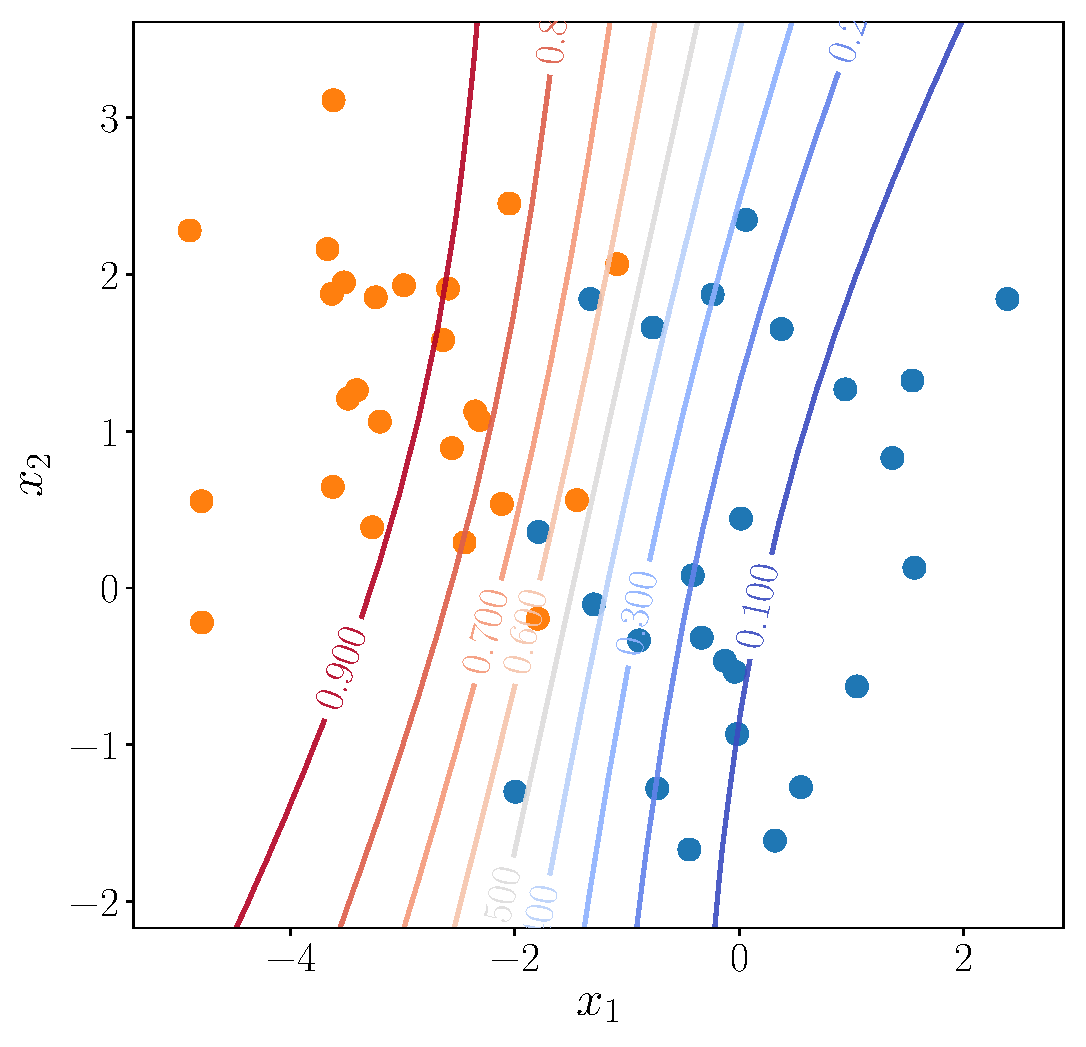
\includegraphics[height=3cm]{./figures/vi/logistic_regression_prediction}
  \end{center}
\end{columns}
\pause
\begin{align*}
    &\text{Prior on model parameter: }p(z) = \gauss{0}{1}\\
    &\text{Likelihood: } p(y_n|x_n, z) = \Ber(\sigma(zx_n))
  \end{align*}
  \vspace{-5mm}
  \pause
  \begin{itemize}
  \item Assume we have a single data point $(x,y)$
  \item Goal: Approximate the intractable posterior distribution $p(z|x,y)$
    using variational inference
  \end{itemize}
\end{frame}

%%%%%%%%%%%%%%%%%%%%%%%%%%%%%%%%%%%%%%
\begin{frame}{Example: Bayesian Logistic Regression (2)}
  \begin{itemize}
  \item Choose Gaussian variational approximation: \\
    $q_\vv(z) = \gauss{z; \mu}{\sigma^2}$ \arrow
    $\vec\nu = \onslide+<2->{\{\mu, \sigma^2\}}$
\onslide+<3->{
  \item Objective function: ELBO $\mathcal F(\vec\nu)$
  \begin{align*}
    \mathcal F(m,\sigma^2) &= \E_q[\orange{\log p(z)}  -\blue{\log 
                             q(z)} + \red{\log
                              p(y|x,z)}]\\
    \onslide+<4->{
                    &  = \orange{-\tfrac{1}{2}(\mu^2 +
                             \sigma^2)} +
                             \blue{\tfrac{1}{2}\log\sigma^2} +  \red{\E_q[\log
                             p(y|x,z)]}  +\text{c}}\\
   \onslide+<5->{\red{\E_q[\log p(y|x,z)]}&=}
\onslide+<6->{\E_q[y\log\sigma(xz)+(1-y)\log(1-\sigma(xz))]}
    \\
    \onslide+<7->{&= \E_q[yxz] - \E_q[y\log(1+\exp(xz))] \\
                         & \quad+
                             \E_q\left[(1-y)\log \left(1 -
                           \frac{\exp(xz)}{1+\exp(xz)}\right)\right]
                           }
  \end{align*}
\onslide+<7->{
  with
  \begin{align*}
    \sigma(xz) &= \frac{\exp(xz)}{1+\exp(xz)}
  \end{align*}
  }
}
\end{itemize}
  
\end{frame}



\begin{frame}{Computing the Expected Log-Likelihood}

  \begin{align*}
  \red{\E_q[\log p(y|x,z)]}&= \E_q[yxz] - \E_q[y\log(1+\exp(xz))] \\
                           &\quad +
                             \E_q[(1-y)\log \left(1 -
                             \frac{\exp(xz)}{1+\exp(xz)}\right)]\\
   \onslide+<2->{ &= yx\mu - \E_q[y\log(1+\exp(xz))]\\&\quad +
                             \E_q[(1-y)\log \left(
    \frac{1}{1+\exp(xz)}\right)]\\}
\onslide+<3->{    &= yx\mu -\E_q[y\log(1+\exp(xz))] \\
                          &\quad
                            - \E_q[\log (1 + \exp(xz))]  + \E_q[y\log
                            (1+ \exp(xz))]\\}
\onslide+<4->{    &=\red{yx\mu - \E_q[\log (1 + \exp(xz))] }}
  \end{align*}
\end{frame}



%%%%%%%%%%%%%%%%%%%%%%%%%%%%%%%%%%%%%%
\begin{frame}{Example: Bayesian Logistic Regression (ctd.)}
  \begin{itemize}
  \item Choose Gaussian variational approximation: \\
    $q_\vv(z) = \gauss{z; \mu}{\sigma^2}$ \arrow
    $\vec\nu = \{\mu, \sigma^2\}$
  \item Objective function: ELBO $\mathcal F(\vec\nu)$
  \end{itemize}
  \begin{align*}
    \mathcal F(\mu,\sigma^2) &= \E_q[\orange{\log p(z)} + \red{\log
                             p(y|x,z)} -\blue{\log 
                             q(z)}]\\
                           &= \orange{-\tfrac{1}{2}(\mu^2 +
                             \sigma^2)} +
                             \blue{\tfrac{1}{2}\log\sigma^2} +  \red{\E_q[\log
                             p(y|x,z)]}  +\text{c}\\
                           &= \orange{-\tfrac{1}{2}(\mu^2 +
                             \sigma^2)} +
                             \blue{\tfrac{1}{2}\log\sigma^2} +
                             \red{yx\mu - \E_q[\log (1 + \exp(xz))] } 
  \end{align*}
  \vspace{-5mm}
  \pause
  \begin{itemize}
  \item \alert{Expectation cannot be computed in closed form}
    % \item \calert{Pushing gradients through Monte Carlo estimates is very hard.}
  \item We want to optimise w.r.t.~variational parameters $\mu, \sigma^2$.
    \pause
  \item How can we optimise quantities that we cannot compute in closed-form?
  \end{itemize}
  
\end{frame}




\begin{frame}{Non-Conjugate Models}

    \begin{itemize}
    \item Nonlinear time series models
    \item Deep latent Gaussian models
    \item Attention models (e.g., DRAW)
    \item Generalized linear models (e.g., logistic regression)
    \item Bayesian neural networks
    \item ...
    \end{itemize}
\pause
    There are many interesting non-conjugate models
    \\\arrow Look for a solution that is not model specific\\
    \arrow \emph{Black-Box Variational Inference}
\end{frame}






\begin{frame}
\begin{center}
\Large \emph{Limitation 2: Large datasets}
\end{center}
\end{frame}


\begin{frame}{Example: Bayesian Logistic Regression}
Usual formulation:
\begin{align}
p(y_n\given \vx_n, \vz) = \mathrm{Ber}(\sigma(\vtheta\transpose\vx_n)) \\
p(\vtheta) = \NormDist{\vtheta; 0, \mathbf{I}}
\end{align}

ELBO:
\begin{align}
\lb &= \Exp{q(\vtheta)}{\log\prod_{n=1}^Np(y_n\given\vx_n,\vtheta)} - \KL{q(\vtheta)}{p(\vtheta)} \nonumber \\
&= \sum_{n=1}^N \Exp{q(\vtheta)}{\log p(y_n\given\vx_n,\vtheta)} - \KL{q(\vtheta)}{p(\vtheta)}
\end{align}
\end{frame}


\begin{frame}{Big data}
\begin{align}
\lb &= \sum_{n=1}^N \Exp{q(\vtheta)}{\log p(y_n\given\vx_n,\vtheta)} - \KL{q(\vtheta)}{p(\vtheta)}
\end{align}

In ``big data'' applications, $N$ may be millions or billions.

\vspace{0.3cm}

\arrow Summing over all datapoints at \emph{each} optimisation iteration for $q(\vtheta)$ is \emph{too slow}.

\end{frame}




\begin{frame}
\begin{center}
\Large \emph{Stochastic Optimisation}
\end{center}
\end{frame}


\begin{frame}{Stochastic Optimisation}




\begin{align}
\lb &= \sum_{n=1}^N \Exp{q(\vtheta)}{\log p(y_n\given\vx_n,\vtheta)} - \KL{q(\vtheta)}{p(\vtheta)}
\end{align}


We can trivially find an \emph{unbiased estimator} of the ELBO and its gradient by subsampling the data points! (solves problem 2)

\pause

\begin{align}
\hat \lb = \frac{N}{M} \sum_{n\in \mathcal{M}} \Exp{q_\vv(\vtheta)}{\log p(y_n\given \vx_n, \vtheta)} - \KL{q_\vv(\vtheta)}{p(\vtheta)} \\
\hat{\pderiv[\lb]{\vv}} = \frac{N}{M} \sum_{n\in \mathcal{M}} \pderiv{\vv} \Exp{q_\vv(\vtheta)}{\log p(y_n\given \vx_n, \vtheta)} - \pderiv{\vv}\KL{q_\vv(\vtheta)}{p(\vtheta)}
\end{align}


\begin{center}
\Large Can we still optimise with estimated gradients? \pause (Yes)
\end{center}


\end{frame}


\begin{frame}{Stochastic Gradient Descent (MML / Comp Opt)}
Goal: $\vv^* = \argmax_\vv \lb(\vv)$
\pause

Normal gradient descent:
\begin{gather}
\vv_t = \vv_{t-1} + \rho_t\nabla_\vv\lb(\vv_{t-1}) \\
\vv_t \to \vv^* \text{ as } t \to \infty
\end{gather}
\pause

Stochastic gradient descent (Robbins \& Monro, 1951):
\begin{gather}
\text{if } \Exp{}{\hat{g}_t} = \nabla_\vv \lb(\vv_{t})
\end{gather}
\vspace{-0.6cm}
\begin{gather}
\vv_t = \vv_{t-1} + \rho_t\hat{g}_t \\
\vv_t \to \vv^* \text{ as } t \to \infty \qquad \qquad \text{if } \sum_{t=1}^\infty\rho_t = \infty \text{ and } \sum_{t=1}^\infty\rho_t^2 < \infty \\
\text{e.g. } \rho_t = 1 / t
\end{gather}

\pause

Having a small $\mathbb{V}\left[\hat g_t\right]$ is crucial to ensure fast convergence.
\end{frame}


\begin{frame}{Stochastic Optimisation}
\begin{itemize}
\item Stochastic optimisation solves problem 2.
\item Still stuck with problem 1: Intractable integrals in VI.
\end{itemize}

\vspace{0.5cm}

\pause

Since we're using stochastic gradient estimates anyway... \pause
\begin{center}
\Large Can we not also find Monte Carlo approximations to the gradients of intractable integrals?
\end{center}
\end{frame}





\begin{frame}
\begin{center}
\Large \emph{Black-Box Variational Inference (BBVI)}
\end{center}
\end{frame}


\begin{frame}{Black-Box Variational Inference}
  \begin{center}
    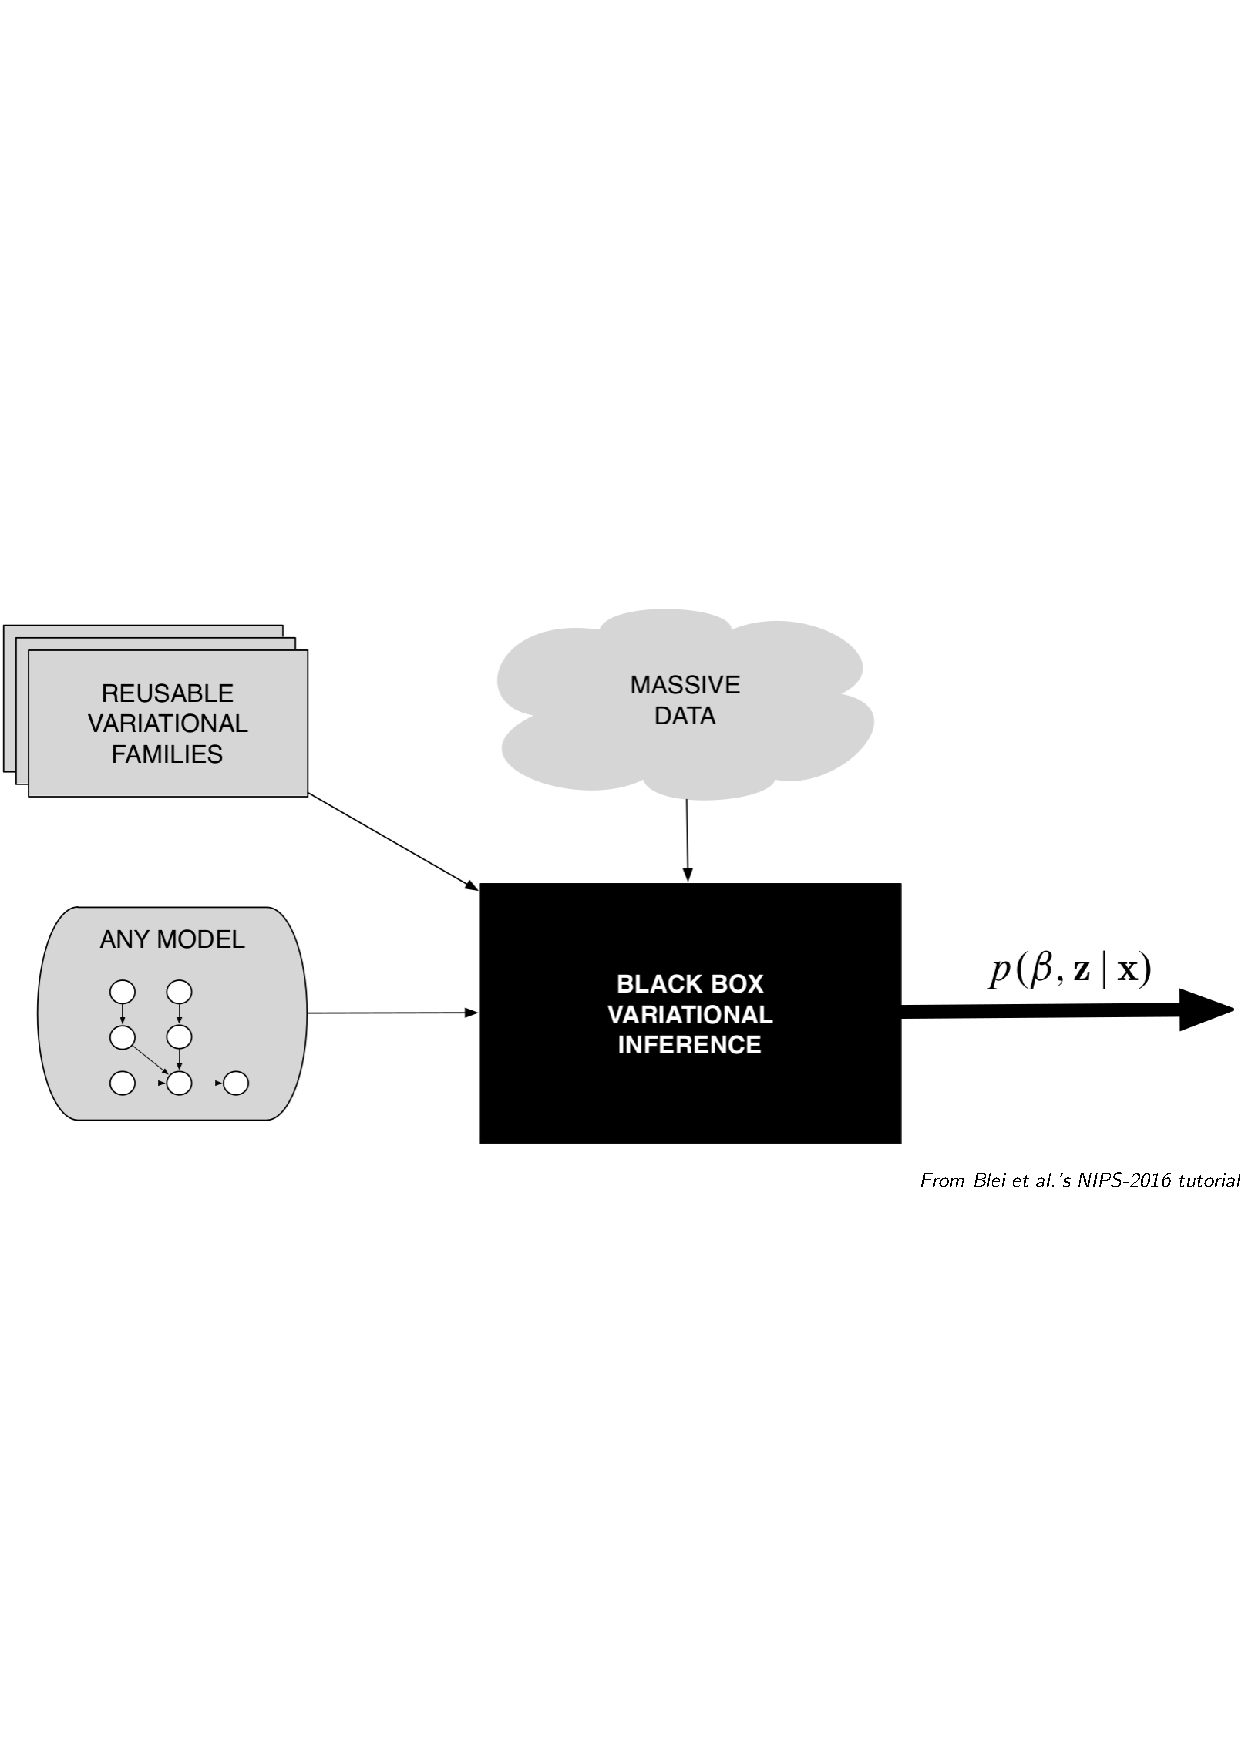
\includegraphics[width=0.8\hsize]{./figures/vi/bbvi}
  \end{center}
  \begin{itemize}
  \item Any model (limitation 1)
  \item Massive data (limitation 2)
  \item Some general assumptions on the approximating family
  \end{itemize}
\end{frame}



\begin{frame}{Black-Box Variational Inference}
Problem 1: Intractable integral of the expected log-likelihood term
\begin{align}
\Exp{q(\vz)}{\log p(\vx\given\vz)} \,.
\end{align}

For stochastic optimisation we need an estimator of its \emph{gradient} $\hat g_t$, such that
\begin{align}
\Exp{}{\hat g_t} = \nabla_\vv \lb(\vv)
\end{align}

\pause
\vspace{0.5cm}

\begin{center}
\Large Can we find such unbiased estimates?
\end{center}

\pause

\begin{itemize}
\item Score function estimator
\item Reparameterisation estimator
\end{itemize}
\end{frame}


\begin{frame}{Problem statement}
We have intractable terms that can be written as:
\begin{align}
\Exp{q_\vv(\vz)}{h(\vz, \vv)}
\end{align}

Goal: Find estimator $\hat g$ with property
\begin{align}
\Exp{}{\hat g} = \nabla_\vv \Exp{q_\vv(\vz)}{h(\vz, \vv)}
\end{align} \pause

Remember:
\begin{itemize}
\item It's easy to find a MC estimate of the objective.
\item But we need an MC estimate of the gradients!
\end{itemize}

\end{frame}


% \begin{frame}{Re-Writing the ELBO}
%   \begin{align*}
%     \text{ELBO} &= \E_q[\log p(\vec x|\vec z)] - \KL{q(\vec
%                   z|\vec\nu)}{p(\vec z)} \\
%   \onslide+<2->{
%     &=\E_q[\blue{\log p(\vec x|\vec z)}] + \E_q[\blue{\log p(\vec z)} - \log q(\vec
%     z|\vec \nu)]\\}
% \onslide+<3->{   & = \E_q[\underbrace{\blue{\log p(\vec x, \vec z)} - \log q(\vec
%      z|\vec\nu)}_{=:h(\vec z, \vec\nu)}]}
%   \end{align*}

%   \onslide+<4->{
%     \begin{myblock}{Evidence Lower Bound}
%       \vspace{-5mm}
% \begin{align*}
%   \text{ELBO}&=\E_q[h(\vec z,\vec\nu)] =  \int h(\vec z, \vec\nu) q(\vec
%                z|\vec\nu)d\vec z\\
%   h(\vec z,\vec\nu) &:= \log p(\vec x, \vec z) - \log
%                       q_\vv(\vec z)
% \end{align*}
% \end{myblock}
% }
% \end{frame}



\begin{frame}[t]{Approach}
\begin{align}
g(\vv) = \nabla_\vv\Exp{q}{h(\vz, \vv)}
\end{align}
% \begin{center}
%     \tikzstyle{ipe stylesheet} = [
  ipe import,
  even odd rule,
  line join=round,
  line cap=butt,
  ipe pen normal/.style={line width=0.4},
  ipe pen heavier/.style={line width=0.8},
  ipe pen fat/.style={line width=1.2},
  ipe pen ultrafat/.style={line width=2},
  ipe pen normal,
  ipe mark normal/.style={ipe mark scale=3},
  ipe mark large/.style={ipe mark scale=5},
  ipe mark small/.style={ipe mark scale=2},
  ipe mark tiny/.style={ipe mark scale=1.1},
  ipe mark normal,
  /pgf/arrow keys/.cd,
  ipe arrow normal/.style={scale=7},
  ipe arrow large/.style={scale=10},
  ipe arrow small/.style={scale=5},
  ipe arrow tiny/.style={scale=3},
  ipe arrow normal,
  /tikz/.cd,
  ipe arrows, % update arrows
  <->/.tip = ipe normal,
  ipe dash normal/.style={dash pattern=},
  ipe dash dashed/.style={dash pattern=on 4bp off 4bp},
  ipe dash dotted/.style={dash pattern=on 1bp off 3bp},
  ipe dash dash dotted/.style={dash pattern=on 4bp off 2bp on 1bp off 2bp},
  ipe dash dash dot dotted/.style={dash pattern=on 4bp off 2bp on 1bp off 2bp on 1bp off 2bp},
  ipe dash normal,
  ipe node/.append style={font=\normalsize},
  ipe stretch normal/.style={ipe node stretch=1},
  ipe stretch normal,
  ipe opacity 10/.style={opacity=0.1},
  ipe opacity 30/.style={opacity=0.3},
  ipe opacity 50/.style={opacity=0.5},
  ipe opacity 75/.style={opacity=0.75},
  ipe opacity opaque/.style={opacity=1},
  ipe opacity opaque,
]
\definecolor{red}{rgb}{1,0,0}%
\begin{tikzpicture}[ipe stylesheet]
  \draw[shift={(311.397, 686.186)}, xscale=0.2262, yscale=0.0959]
    (0, 0)
     .. controls (10.6667, 26.6667) and (58.6667, 74.6667) .. (109.3333, 69.3333)
     .. controls (160, 64) and (213.3333, 5.3333) .. (234.6667, -50.6667)
     .. controls (256, -106.6667) and (245.3333, -160) .. (208, -200)
     .. controls (170.6667, -240) and (106.6667, -266.6667) .. (88, -248)
     .. controls (69.3333, -229.3333) and (96, -165.3333) .. (96, -122.6667)
     .. controls (96, -80) and (69.3333, -58.6667) .. (42.6667, -45.3333)
     .. controls (16, -32) and (-10.6667, -26.6667) .. cycle;
  \pic
     at (339.3985, 680.6362) {ipe disk};
  \draw[shift={(339.398, 680.636)}, scale=0.1686, -{>[ipe arrow small]}]
    (0, 0)
     .. controls (48, 16) and (112, -48) .. (158.005, -9.169);
  \pic
     at (366.0336, 679.0905) {ipe disk};
  \node[ipe node]
     at (84, 708) {$p(\vec x, \vec z)$};
  \node[ipe node]
     at (84, 648) {$q(\vec z|\vec \nu)$};
  \draw[shift={(196, 696)}, xscale=1.25,  ipe pen fat]
    (0, 0) rectangle (64, -32);
  \node[ipe node]
     at (204.891, 677.511) {$\displaystyle \int (...) q(\vec z|\vec
       \nu) d\vec z$};
  \node[ipe node]
     at (141.371, 677.339) {$\nabla_{\vec \nu}$};
  \draw[ipe pen fat]
    (132, 696) rectangle (164, 664);
  \draw[->]
    (164, 680)
     -- (196, 680);
  \draw[->]
    (276, 680)
     -- (308, 680);
  \draw[->]
    (112, 656)
     -- (132, 664);
  \draw[->]
    (112, 704)
     -- (132, 696);
  \node[ipe node, font=\tiny]
     at (245, 646.47) {\it \sffamily Adopted from Blei et al.'s NIPS-2016 tutorial};
\end{tikzpicture}

%%% Local Variables:
%%% mode: latex
%%% TeX-master: "../lecture_variational_inference"
%%% End:

%   \end{center}
  \begin{itemize}[<+->]
    \item Switch order to integration first, then differentiation \\
(Monte Carlo estimates need expectations, and expectations are integrals)
    \item Write integration as expectation again
    \item Approximate the expectation after having taken the gradient\newline
      \arrow Monte Carlo estimator (ideally with low variance)
    \item Stochastic optimization
    \end{itemize}
    \onslide+<5->{
    \arrow Require: \cemph{general way to compute gradients of
      expectations}}
\end{frame}



\begin{frame}{Log-Derivative Trick}
  \begin{myblock2}{Log-Derivative Trick}
\vspace{-2mm}
    \begin{align*}
      &\nabla_{\vec\nu} \log q_\vv(\vec z) = 
      \onslide+<2->{\frac{\nabla_{\vec\nu}q_\vv(\vec z)}{q_\vv(\vec z)}\\
      \iff & \nabla_{\vec\nu}q_\vv(\vec z) = q_\vv(\vec
             z)\nabla_{\vec\nu} \log q_\vv(\vec z) }
    \end{align*}
  \end{myblock2}
  \onslide+<3->{
  \begin{itemize}
    \item 
  Therefore:
  \begin{align*}
    \int \nabla_{\vec\nu} q_\vv(\vec z) f(\vec z) d\vec z &= \int q_\vv(\vec
             z)\nabla_{\vec\nu} \log q_\vv(\vec z) f(\vec z)d\vec z \\
    &= \E_q[\nabla_{\vec\nu} \log q_\vv(\vec z) f(\vec z)]
  \end{align*}
}
\vspace{-5mm}
\onslide+<4->{
    \item If we can sample from $q$, this expectation can be evaluated
      easily (Monte Carlo estimation)
    \end{itemize}
    }
\end{frame}






\begin{frame}{Gradients of Expectations: Approach 1}
  $$
  \text{ELBO} = \mathcal F(\vec\nu) = \E_q[h(\vec z,\vec\nu)]\,,\quad
  h(\vec z, \vec\nu) = \log p(\vec x, \vec z) - \log q(\vec
     z|\vec\nu)
     $$
     \vspace{-5mm}
  \begin{itemize}
    \item Need gradient of ELBO w.r.t. variational parameters $\vec\nu$
  \end{itemize}
\onslide+<2->{
  \begin{align*}
    \nabla_{\vec\nu}&\mathcal F =\blue{\nabla_{\vec\nu} \E_q[h(\vec
                      z,\vec\nu)]}
                      \onslide<3->{
                      = \nabla_{\vec\nu}\int h(\vec z, \vec\nu)
                      q_\vv(\vec z)d\vec z\\}
    \onslide<4->{
                    &= \int \big(\nabla_{\vec\nu} h(\vec\nu, \vec z)\big) q_\vv(\vec z) +
                      \orange{h(\vec\nu, \vec z)\nabla_{\vec\nu}q_\vv(\vec z)}d\vec z
                      \qquad\hspace{9mm}\fbox{product rule}\\
    }
    \onslide<5->{
                    &= \int 
                      q_\vv(\vec z)\nabla_{\vec\nu}h(\vec z,
                      \vec\nu) + \orange{q_\vv(\vec z) \nabla_{\vec\nu}\log q_\vv(\vec z)
                      h(\vec z, \vec \nu)}  d\vec
                      z\quad\fbox{log-deriv. trick}\\
    }
                    &= \blue{\E_q[\nabla_{\vec\nu} \log q(\vec z|\vec \nu)h(\vec z,\vec\nu)
                      + \nabla_{\vec\nu}h(\vec z,\vec\nu)]}
  \end{align*}
}
\vspace{-6mm}
  \onslide+<6->{
  \begin{itemize}
    \item We successfully \cemph{swapped gradient and expectation}
    \item $q$ known\newline
      \arrow Sample from $q$ and use Monte Carlo estimation
    \end{itemize}
  }
\end{frame}



\begin{frame}{Score Function}
  \begin{itemize}[<+->]
  \item \cemph{Score function:} Derivative of a log-likelihood
    with respect to the parameter vector $\vec\nu$:
    \begin{myblock}{Score Function}
      \vspace{-5mm}
    \begin{align*}
      \text{score} = \nabla_{\vec\nu} \log q_\vv(\vec z) =
      \frac{1}{q_\vv(\vec z)}\nabla_{\vec\nu}q_\vv(\vec z)
    \end{align*}
  \end{myblock}
\item Measures the sensitivity of the log-likelihood
    w.r.t. $\vec\nu$
  % \item Central to maximum likelihood estimation
  \end{itemize}
  
\end{frame}



%%%%%%%%%%%%%%%%%%%%%%%%%%%%%%%%%
\begin{frame}{Score Function (2)}
  \begin{align*}
  \text{score} = \nabla_{\vec\nu} \log q_\vv(\vec z) =
  \frac{1}{q_\vv(\vec z)}\nabla_{\vec\nu}q_\vv(\vec z)
  \end{align*}
  
  \begin{itemize}
  \item Important property:
    \begin{align*}
      \E_{q_\vv(\vec z)}[\text{score}] &= \onslide+<2->{\E_{q_\vv(\vec z)}
                                  \left[\frac{1}{q_\vv(\vec z)}\nabla_{\vec\nu}q_\vv(\vec z)\right] \\
                                &= \int
                                  \frac{1}{q_\vv(\vec z)} q_\vv(\vec z)\nabla_{\vec\nu}q_\vv(\vec z) d\vec z\\
                                &= \int \nabla_{\vec\nu}q_\vv(\vec z)d\vec z =
                                  \nabla_{\vec\nu} \int q_\vv(\vec z) d\vec z = \nabla_{\vec
                                  \nu} 1 = 0}
    \end{align*}
    \onslide+<2->{\arrow \cemph{Mean of the score function is $0$}}
    \pause
  % \item Variance of the score: \cemph{Fisher information} \arrow
  \end{itemize}
\end{frame}




\begin{frame}{Score Function Gradient Estimator}
  $$\text{ELBO} = \E_q[h(\vec z,\vec\nu)] =
  \E_q[\log p(\vec x, \vec z) - \log q_\vv(\vec z)]$$
  \vspace{-6mm}
  \begin{itemize}
    \item Gradient of ELBO:
  \begin{align*}
    \nabla_{\vec\nu} \text{ELBO} &= \onslide+<2->{\E_q[\nabla_{\vec\nu} \log q_\vv(\vec z)h(\vec z,\vec\nu)] +
    \E_q[\orange{\nabla_{\vec\nu} h(\vec z,\vec\nu)}]\\}
\onslide+<3->{    &= \E_q[\nabla_{\vec\nu} \log q_\vv(\vec z)h(\vec z,\vec\nu)]\\
    &\quad + \E_q[\orange{\underbrace{\nabla_{\vec\nu}\log p(\vec x, \vec
      z)}_{=0} - \underbrace{\nabla_{\vec\nu} \log q_\vv(\vec 
      z)}_{\text{score}}}]}
  \end{align*}
  \onslide+<4->{
    \vspace{-3mm}
\item Exploit that the mean of the score function is $0$. Then:
  \begin{align*}
    \nabla_{\vec\nu} \text{ELBO} & = \E_q[\nabla_{\vec\nu} \log q_\vv(\vec z)h(\vec z,\vec\nu)] \\
    &= \E_q[\nabla_{\vec\nu}\log q_\vv(\vec z)(\log p(\vec x, \vec z) -
      \log q_\vv(\vec z)) ]
  \end{align*}
}%
\vspace{-6mm}
\onslide+<5->{%
  \item \cemph{Likelihood ratio gradient} (Glynn, 1990)
  \item \cemph{REINFORCE gradient} (Williams, 1992)%\nocite{Williams1992}
  }
\end{itemize}
\end{frame}

  
% \end{frame}
%%%%%%%%%%%%%%%%%%%%%%%%%%%%%%%%%
\begin{frame}{Using Noisy Stochastic Gradients}
  \begin{itemize}[<+->]
    \item Gradient of the ELBO
  \begin{align*}
    \nabla_{\vec\nu}\text{ELBO} = \E_q[\nabla_{\vec\nu}\log q_\vv(\vec z) (\log p(\vec x, \vec z) - \log q_\vv(\vec z))]
  \end{align*}
  is an expectation
  \item Require that $q_\vv(\vec z)$ is differentiable
    w.r.t. $\vec\nu$
\item Get noisy unbiased gradients using Monte Carlo by sampling from $q$:
  \begin{align*}
    \frac{1}{S}\sum_{s=1}^S \nabla_{\vec\nu}\log q_\vv(\vec z\idx{s}) (\log p(\vec x, \vec z\idx{s}) - \log q_\vv(\vec z\idx{s}))\,,\quad \vec z\idx{s} \sim q_\vv(\vec z)
  \end{align*}
\item Sampling from $q$ is easy (we choose $q$)
\item Use this within SVI to converge to a local optimum
\end{itemize}
\end{frame}









\begin{frame}{Summary: BBVI procedure}
Black Box Variational Inference

  \begin{enumerate}
    \item Input: model $p(\vec x, \vec z)$, variational approximation
      $q_\vv(\vec z)$
    \item Repeat
      \begin{enumerate}
      \item Draw $S$ samples $\vec z\idx{s}\sim q_\vv(\vec z)$
      \item Update variational parameters
        $$
        \vec\nu_{t+1} = \vec\nu_t + \rho_t \underbrace{\orange{\frac{1}{S}\sum_{s=1}^S \nabla_{\vec\nu}\log q(\vec
    z\idx{s}|\vec\nu) (\log p(\vec x, \vec z^{\idx{s}}) - \log q(\vec
    z\idx{s}|\vec\nu))}}_{\text{MC estimate of the score-function gradient of the ELBO}}
    $$
    \item $t=t+1$
    \end{enumerate}
  \end{enumerate}
\end{frame}




\begin{frame}{Requirements for Inference}
Similar to MCMC in that it makes \emph{few} requirements
  \begin{itemize}
  \item Computing the noisy gradient of the ELBO requires:
    \begin{itemize}
    \item Sampling from $q$. We choose $q$ so that this is possible.
    \item Evaluate the score function
      $\nabla_{\vec\nu}\log q_\vv(\vec z)$
    \item Evaluate $\log q_\vv(\vec z)$ and
      $\log p(\vec x, \vec z) = \log p(\vec z) + \log p(\vec x|\vec
      z)$
    \end{itemize}
    \arrow \cemph{No model-specific computations for optimization}
    (computations are only specific to the choice of the variational approximation)
  \end{itemize}

\end{frame}




\begin{frame}{Issue: Variance of the Gradients}
  \begin{itemize}
    \item Stochastic optimization \arrow \alert{Gradients are noisy (high variance)}
    \item The noisier the gradients, the slower the convergence
    \item Possible solutions:
      \begin{itemize}
      \item \cemph{Control variates} (with the score function as control variate)
      \item \cemph{Rao-Blackwellization}
      \item \cemph{Importance sampling}
      \end{itemize}
    \end{itemize}

\end{frame}



\begin{frame}{Issues with score function estimator}
  We can simplify the gradient estimator further:
  \begin{itemize}
    \item Score-function gradient estimator only requires general
      assumptions
    \item Noisy gradients are a problem
    \item Address this issue by making some additional assumptions
      (not too strict) \newline
      \arrow \cemph{Pathwise gradient estimators}
  \end{itemize}
\end{frame}


\begin{frame}[t]{Approach}
\begin{align}
g(\vv) = \nabla_\vv\Exp{q}{h(\vz, \vv)}
\end{align}
% \begin{center}
%     \tikzstyle{ipe stylesheet} = [
  ipe import,
  even odd rule,
  line join=round,
  line cap=butt,
  ipe pen normal/.style={line width=0.4},
  ipe pen heavier/.style={line width=0.8},
  ipe pen fat/.style={line width=1.2},
  ipe pen ultrafat/.style={line width=2},
  ipe pen normal,
  ipe mark normal/.style={ipe mark scale=3},
  ipe mark large/.style={ipe mark scale=5},
  ipe mark small/.style={ipe mark scale=2},
  ipe mark tiny/.style={ipe mark scale=1.1},
  ipe mark normal,
  /pgf/arrow keys/.cd,
  ipe arrow normal/.style={scale=7},
  ipe arrow large/.style={scale=10},
  ipe arrow small/.style={scale=5},
  ipe arrow tiny/.style={scale=3},
  ipe arrow normal,
  /tikz/.cd,
  ipe arrows, % update arrows
  <->/.tip = ipe normal,
  ipe dash normal/.style={dash pattern=},
  ipe dash dashed/.style={dash pattern=on 4bp off 4bp},
  ipe dash dotted/.style={dash pattern=on 1bp off 3bp},
  ipe dash dash dotted/.style={dash pattern=on 4bp off 2bp on 1bp off 2bp},
  ipe dash dash dot dotted/.style={dash pattern=on 4bp off 2bp on 1bp off 2bp on 1bp off 2bp},
  ipe dash normal,
  ipe node/.append style={font=\normalsize},
  ipe stretch normal/.style={ipe node stretch=1},
  ipe stretch normal,
  ipe opacity 10/.style={opacity=0.1},
  ipe opacity 30/.style={opacity=0.3},
  ipe opacity 50/.style={opacity=0.5},
  ipe opacity 75/.style={opacity=0.75},
  ipe opacity opaque/.style={opacity=1},
  ipe opacity opaque,
]
\definecolor{red}{rgb}{1,0,0}%
\begin{tikzpicture}[ipe stylesheet]
  \draw[shift={(311.397, 686.186)}, xscale=0.2262, yscale=0.0959]
    (0, 0)
     .. controls (10.6667, 26.6667) and (58.6667, 74.6667) .. (109.3333, 69.3333)
     .. controls (160, 64) and (213.3333, 5.3333) .. (234.6667, -50.6667)
     .. controls (256, -106.6667) and (245.3333, -160) .. (208, -200)
     .. controls (170.6667, -240) and (106.6667, -266.6667) .. (88, -248)
     .. controls (69.3333, -229.3333) and (96, -165.3333) .. (96, -122.6667)
     .. controls (96, -80) and (69.3333, -58.6667) .. (42.6667, -45.3333)
     .. controls (16, -32) and (-10.6667, -26.6667) .. cycle;
  \pic
     at (339.3985, 680.6362) {ipe disk};
  \draw[shift={(339.398, 680.636)}, scale=0.1686, -{>[ipe arrow small]}]
    (0, 0)
     .. controls (48, 16) and (112, -48) .. (158.005, -9.169);
  \pic
     at (366.0336, 679.0905) {ipe disk};
  \node[ipe node]
     at (84, 708) {$p(\vec x, \vec z)$};
  \node[ipe node]
     at (84, 648) {$q(\vec z|\vec \nu)$};
  \draw[shift={(196, 696)}, xscale=1.25,  ipe pen fat]
    (0, 0) rectangle (64, -32);
  \node[ipe node]
     at (204.891, 677.511) {$\displaystyle \int (...) q(\vec z|\vec
       \nu) d\vec z$};
  \node[ipe node]
     at (141.371, 677.339) {$\nabla_{\vec \nu}$};
  \draw[ipe pen fat]
    (132, 696) rectangle (164, 664);
  \draw[->]
    (164, 680)
     -- (196, 680);
  \draw[->]
    (276, 680)
     -- (308, 680);
  \draw[->]
    (112, 656)
     -- (132, 664);
  \draw[->]
    (112, 704)
     -- (132, 696);
  \node[ipe node, font=\tiny]
     at (245, 646.47) {\it \sffamily Adopted from Blei et al.'s NIPS-2016 tutorial};
\end{tikzpicture}

%%% Local Variables:
%%% mode: latex
%%% TeX-master: "../lecture_variational_inference"
%%% End:

%   \end{center}
  \begin{itemize}[<+->]
    \item Switch order to integration first, then differentiation
    \item Write integration as expectation again
    \item Approximate the expectation after having taken the gradient\newline
      \arrow Monte Carlo estimator (ideally with low variance)
    \item Stochastic optimization
    \end{itemize}
    \onslide+<5->{
    \arrow Require: \cemph{general way to compute gradients of
      expectations}}
\end{frame}



\begin{frame}{Change of Variables}
Some distributions can be sampled using a \emph{change of variables}, i.e.
\begin{gather*}
\vz = \vec t(\vepsilon) \qquad \text{with } \vepsilon \sim p(\vepsilon)
\implies p(\vz) \text{ some desired distribution}
\end{gather*}
Densities are related
\begin{gather*}
p(\vepsilon) = p(\vz = t(\vepsilon)) \pderiv[t(\vepsilon)]{\vepsilon}
\end{gather*}
Integrals are related
\begin{gather*}
\int h(\vz) p(\vz) \calcd{\vz} = \int h(t(\vepsilon)) p(\vz = t(\vepsilon)) \pderiv[t(\vepsilon)]{\vepsilon} \calcd{\vepsilon} = \int h(t(\vepsilon)) p(\vepsilon) \calcd{\vepsilon}
\end{gather*}
  \begin{center}
  \tikzstyle{ipe stylesheet} = [
  ipe import,
  even odd rule,
  line join=round,
  line cap=butt,
  ipe pen normal/.style={line width=0.4},
  ipe pen heavier/.style={line width=0.8},
  ipe pen fat/.style={line width=1.2},
  ipe pen ultrafat/.style={line width=2},
  ipe pen normal,
  ipe mark normal/.style={ipe mark scale=3},
  ipe mark large/.style={ipe mark scale=5},
  ipe mark small/.style={ipe mark scale=2},
  ipe mark tiny/.style={ipe mark scale=1.1},
  ipe mark normal,
  /pgf/arrow keys/.cd,
  ipe arrow normal/.style={scale=7},
  ipe arrow large/.style={scale=10},
  ipe arrow small/.style={scale=5},
  ipe arrow tiny/.style={scale=3},
  ipe arrow normal,
  /tikz/.cd,
  ipe arrows, % update arrows
  <->/.tip = ipe normal,
  ipe dash normal/.style={dash pattern=},
  ipe dash dashed/.style={dash pattern=on 4bp off 4bp},
  ipe dash dotted/.style={dash pattern=on 1bp off 3bp},
  ipe dash dash dotted/.style={dash pattern=on 4bp off 2bp on 1bp off 2bp},
  ipe dash dash dot dotted/.style={dash pattern=on 4bp off 2bp on 1bp off 2bp on 1bp off 2bp},
  ipe dash normal,
  ipe node/.append style={font=\normalsize},
  ipe stretch normal/.style={ipe node stretch=1},
  ipe stretch normal,
  ipe opacity 10/.style={opacity=0.1},
  ipe opacity 30/.style={opacity=0.3},
  ipe opacity 50/.style={opacity=0.5},
  ipe opacity 75/.style={opacity=0.75},
  ipe opacity opaque/.style={opacity=1},
  ipe opacity opaque,
]
\definecolor{red}{rgb}{1,0,0}%
\definecolor{green}{rgb}{0,1,0}%
\definecolor{blue}{rgb}{0,0,1}%
\definecolor{yellow}{rgb}{1,1,0}%
\definecolor{orange}{rgb}{1,0.647,0}%
\definecolor{gold}{rgb}{1,0.843,0}%
\definecolor{purple}{rgb}{0.627,0.125,0.941}%
\definecolor{gray}{rgb}{0.745,0.745,0.745}%
\definecolor{brown}{rgb}{0.647,0.165,0.165}%
\definecolor{navy}{rgb}{0,0,0.502}%
\definecolor{pink}{rgb}{1,0.753,0.796}%
\definecolor{seagreen}{rgb}{0.18,0.545,0.341}%
\definecolor{turquoise}{rgb}{0.251,0.878,0.816}%
\definecolor{violet}{rgb}{0.933,0.51,0.933}%
\definecolor{darkblue}{rgb}{0,0,0.545}%
\definecolor{darkcyan}{rgb}{0,0.545,0.545}%
\definecolor{darkgray}{rgb}{0.663,0.663,0.663}%
\definecolor{darkgreen}{rgb}{0,0.392,0}%
\definecolor{darkmagenta}{rgb}{0.545,0,0.545}%
\definecolor{darkorange}{rgb}{1,0.549,0}%
\definecolor{darkred}{rgb}{0.545,0,0}%
\definecolor{lightblue}{rgb}{0.678,0.847,0.902}%
\definecolor{lightcyan}{rgb}{0.878,1,1}%
\definecolor{lightgray}{rgb}{0.827,0.827,0.827}%
\definecolor{lightgreen}{rgb}{0.565,0.933,0.565}%
\definecolor{lightyellow}{rgb}{1,1,0.878}%
\definecolor{black}{rgb}{0,0,0}%
\definecolor{white}{rgb}{1,1,1}%
%%% Local Variables:
%%% mode: latex
%%% TeX-master: t
%%% End:

\begin{tikzpicture}[ipe stylesheet]
  \fill[blue!40!white]
    (128, 736) rectangle (160, 704);
  \fill[orange!40!white]
    (320, 704)
     -- (256, 736)
     -- (288, 768)
     -- (352, 736)
     -- (320, 704);
  \draw[ipe pen ultrafat, -{>[ipe arrow small]}]
    (320, 704)
     -- (256, 736);
  \draw[ipe pen ultrafat, -{>[ipe arrow small]}]
    (320, 704)
     -- (352, 736);
  \draw[ipe pen ultrafat, -{>[ipe arrow small]}]
    (128, 704)
     -- (160, 704);
  \draw[ipe pen ultrafat, -{>[ipe arrow small]}]
    (128, 704)
     -- (128, 736);
  \node[ipe node]
     at (140, 692) {$\vec b_1$};
  \node[ipe node]
     at (112, 720) {$\vec b_2$};
  \node[ipe node]
     at (260, 720) {$\vec c_1$};
  \node[ipe node]
     at (348, 720) {$\vec c_2$};
  \draw[ipe pen heavier, -{>[ipe arrow small]}]
    (176, 736)
     arc[start angle=-129.0939, end angle=-75.9638, x radius=82.4621, y radius=-82.4621];
  \node[ipe node]
     at (204, 736) {$\vec t(\cdot)$};
\end{tikzpicture}

%%% Local Variables:
%%% mode: latex
%%% TeX-master: "../mml-book"
%%% End:

\end{center}
% \begin{itemize}
%   \item Use function $\vec
%     \vepsilon\mapsto \vec t(\vec \epsilon) = \vec \vz$
%   \item Gives new density
%     \begin{align}
%       p(\vz) = p(\vepsilon = \vec t\inv(\vz))
%     \end{align}
%   \end{itemize}
\end{frame}




\begin{frame}{Gradients of Expectations: Approach 2}
  \begin{align*}
    \nabla_{\vec\nu}\text{ELBO} &= \blue{\nabla_{\vec\nu}\E_q[g(\vec
                                  z, \vec\nu)]} \\
                                \onslide+<2->{&= \nabla_{\vec\nu}\int
                                  g(\vec z, \vec\nu) q_\vv(\vec z) d\vec z\\}
                                \onslide+<3->{&=\nabla_{\vec\nu}\int g(\vec z, \vec\nu)
                                  q(\vec\epsilon)d\vec\epsilon \qquad\qquad
                                  \fbox{$q(\vec z) d\vec z = q(\vec\epsilon)d\vec\epsilon$}\\}
                                \onslide+<4->{&= \nabla_{\vec\nu}\int g(t(\vec
                                  \epsilon, \vec\nu),
                                  \vec\nu)q(\vec\epsilon)d\vec\epsilon\qquad\fbox{$\vec z =
                                  t(\vec \epsilon, \vec\nu)$}\\}
                                \onslide+<5->{&= \int \nabla_{\vec\nu} g(t(\vec\epsilon,
                                  \vec\nu), \vec\nu){q(\vec\epsilon)}d\vec\epsilon\qquad
                                  \fbox{$\nabla_{\vec\nu}\int_{\vec\epsilon}
                                  = \int_{\vec\epsilon}\nabla_{\vec\nu}$}\\}
                                \onslide+<6->{&= \blue{\E_{q(\vec\epsilon)}[\nabla_{\vec\nu}g( t(\vec\epsilon,\vec\nu), \vec\nu)]}}
  \end{align*}
\onslide+<7->{\arrow Turned gradient of an expectation into
  expectation of a gradient (and sampling from $q(\vec\epsilon)$ is
  very easy).}
\end{frame}






\begin{frame}{Reparametrization Trick}


  \begin{myblock2}{Reparametrization Trick}
    Base distribution $p(\vec\epsilon)$ and a deterministic
    transformation $\vec z = t(\vec\epsilon, \vec\nu)$ so that $ \vec
    z \sim q_\vv(\vec z)$. Then:
    \begin{align*}
      \nabla_{\vec\nu}\E_{q_\vv(\vec z)}[f(\blue{\vec z})] =
      \E_{p(\vec\epsilon)}[\nabla_{\vec\nu}f(\blue{t(\vec\epsilon, \vec\nu)})]
    \end{align*}
    \arrow Expectation taken w.r.t. base distribution
  %  \arrow We can swap differentiation and integration
  \end{myblock2}
\pause
  \begin{itemize}
    \item Key idea: change of variables using a deterministic transformation
  \end{itemize}
\end{frame}

%%%%%%%%%%%%%%%%%%%%%%% 
\begin{frame}{Example}
  \begin{figure}
    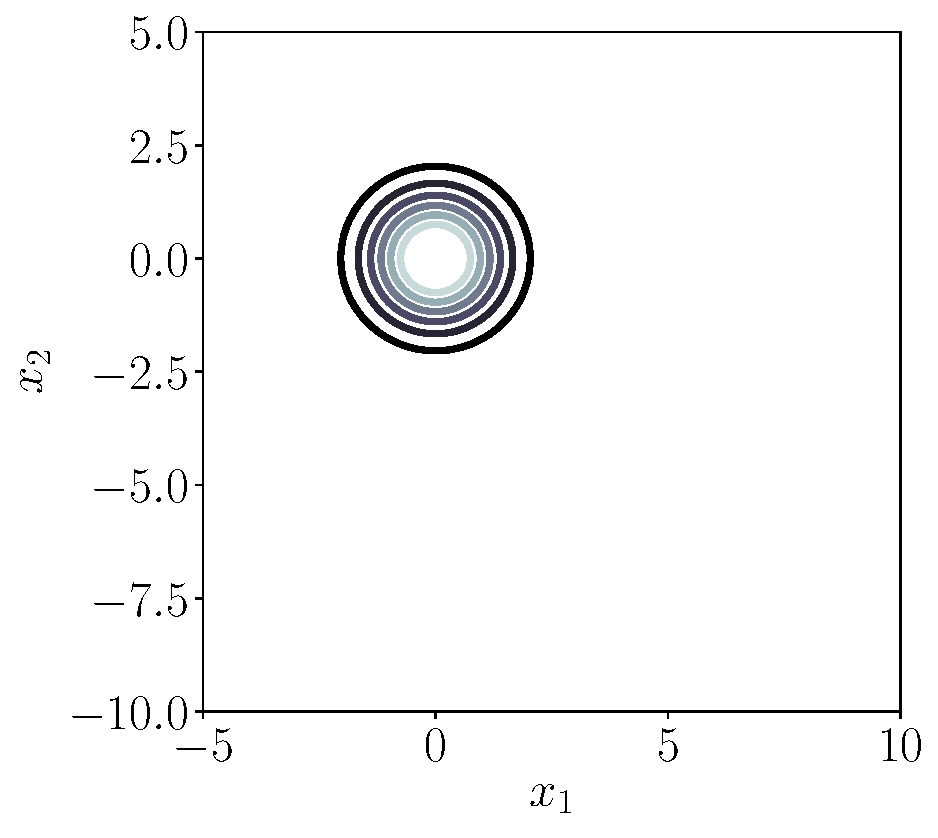
\includegraphics[width=0.4\hsize]{./figures/vi/standard_normal}
    \hspace{2mm}
    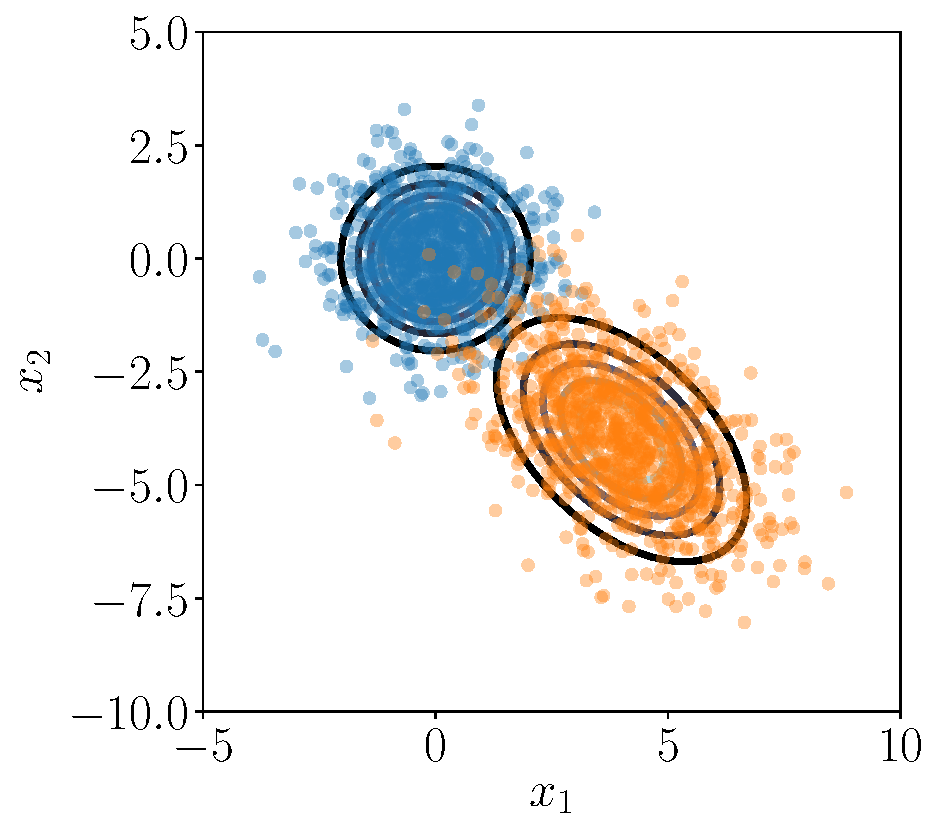
\includegraphics[width=0.4\hsize]{./figures/vi/reparam_trick_example}
  \end{figure}
  \begin{align*}
    \vec\nu &:=\{\vec\mu, \mat R\}\,,\quad \mat R\mat R\T = \mat\Sigma\\
    p(\vec\epsilon) &= \gauss{\vec 0}{\mat I}\\
    t(\vec\epsilon, \vec\nu) &= \vec\mu + \mat R\vec\epsilon\\
    \implies p(\vec z) &= \gaussx{\vec z}{\vec\mu}{\mat\Sigma}
  \end{align*}
  \begin{itemize}
  \item Base distribution is parameter free
  \item Simple deterministic transformation $t$ generate more
    expressive distributions\footnote{\url{https://tinyurl.com/hyakoj2}}
  \end{itemize}
  
\end{frame}



\begin{frame}{Pathwise Gradients}
\begin{align*}
    g(\vec z , \vec \nu) &= \log p(\vec x, \vec z) - \log q(\vec
    z|\vec\nu)\\
  \vec z &= t(\vec \epsilon, \vec\nu)
  \end{align*}
  %
  Simplify gradient of the ELBO:
  \pause
  \begin{align*}
    \nabla_{\vec\nu}&\text{ELBO}= \E_{p(\vec\epsilon)}[\nabla_{\vec\nu} g(t(\vec\epsilon, \vec\nu),
                                 \vec\nu)]\\
                               &=
                                 \E_{p(\vec\epsilon)}[\blue{\nabla_{\vec\nu} \log  p(\vec x,
                                 t(\vec\epsilon,\vec\nu))} -
                                 \orange{\nabla_{\vec\nu} \log
                                 q(t(\vec\epsilon,\vec\nu)|\vec\nu)}]\quad\fbox{Def. of
                                 $g$}\\
                               &= \E_{p(\vec\epsilon)}[\blue{\nabla_{\vec z}\log p(\vec x, \vec
                                 z) \nabla_{\vec\nu}
                                 t(\vec\epsilon,\vec\nu
                                 )}\\
                               &\quad -
                                 \orange{\nabla_{\vec z} \log q(\vec
                                 z|\vec\nu)\nabla_{\vec \nu}t(\vec \epsilon,\vec\nu)
                                 -\underbrace{\nabla_{\vec\nu}\log q(t(\vec\epsilon,\vec\nu)|\vec\nu)}_{\text{score}}}]\quad\fbox{Chain rule}\\
                               &=\E_{p(\vec\epsilon)}[\nabla_{\vec z}\big(\log p(\vec x, \vec z) -\log
                                 q_\vv(\vec z)\big)\nabla_{\vec\nu}
                                 t(\vec\epsilon, \vec\nu)]\quad\hspace{3mm} \fbox{Score property}
  \end{align*}
  \vspace{-4mm}
  \begin{itemize}
  \item \cemph{Pathwise gradient}
  \item \cemph{Reparametrization gradient}
  \end{itemize}
\end{frame}



\begin{frame}{Variance Comparison}
  \begin{figure}
    \centering
    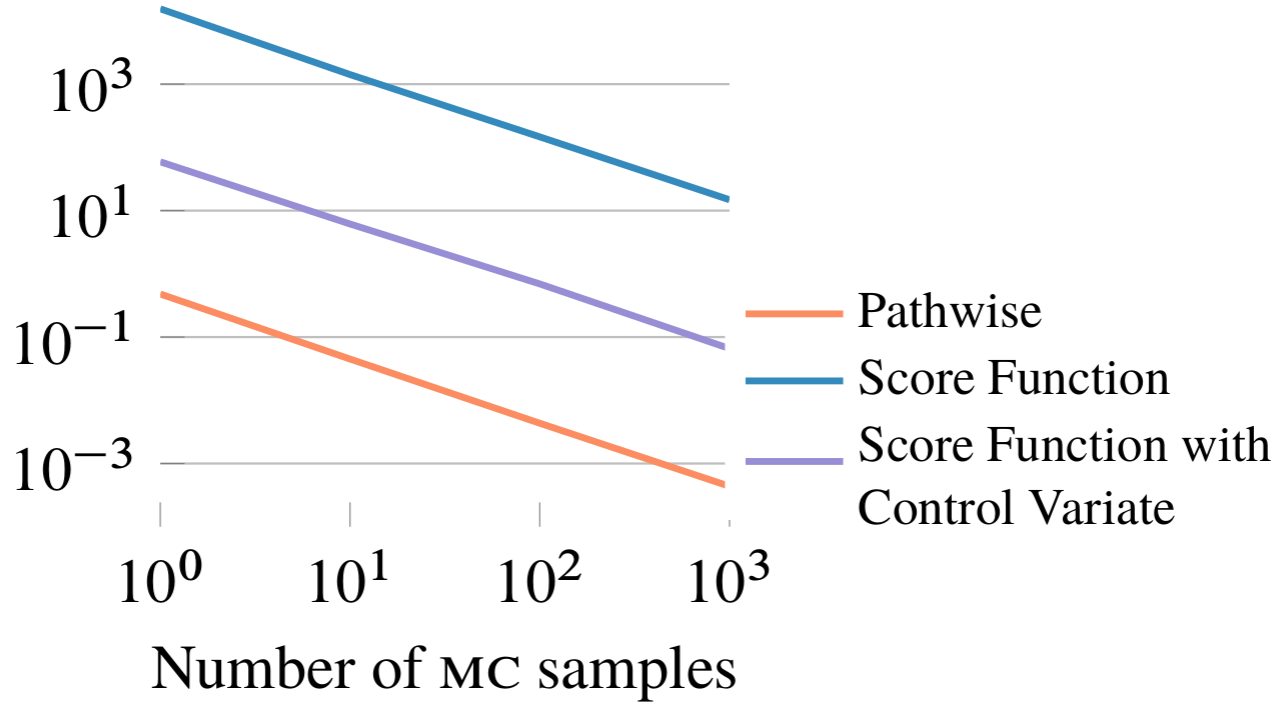
\includegraphics[height=3cm]{./figures/vi/var_comp_score_rep}
  \end{figure}
  \begin{itemize}[<+->]
    \item Drastically reduced variance compared to score-function
      gradient estimation
    \item Restricted class of models (compared with score function
      estimator)
  \end{itemize}
\end{frame}



\begin{frame}{Score Function vs Pathwise
    Gradients}
  \begin{myblock}{}
    \vspace{-5mm}
  \begin{align*}
    \text{ELBO} &= \int g(\vec z, \vec\nu) q_\vv(\vec z)d\vec z\\
    g(\vec z, \vec\nu) &= \log p(\vec x, \vec z) - \log q(\vec z|\vec\mu)
  \end{align*}
\end{myblock}
\begin{itemize}
  \item Score function gradient:
    $$
\nabla_{\vec\nu}\text{ELBO} = \E_q[\blue{\big(\nabla_{\vec\nu}\log q(\vec
z|\vec\nu)\big)} g(\vec z, \vec\nu)]
$$
\arrow Gradient of the variational distribution
  \item Reparametrization gradient:
    $$
\nabla_{\vec\nu}\text{ELBO} =\E_{p(\vec\epsilon)}[\blue{\big(\nabla_{\vec
    z}g(\vec z,\vec\nu)\big)}\nabla_{\vec\nu}
      t(\vec\epsilon, \vec\nu)]
      $$
      \arrow Gradient of the model and the variational distribution
    \item Often, $\Exp{q_\vv(\vz)}{\log q_\vv(\vz)}$ can be computed in closed form, and is excluded from MC estimation. (Skill to recognise when.)
  \end{itemize}
  
\end{frame}


\begin{frame}{Summary}

  \begin{itemize}
  \item Score function
    \begin{itemize}
    \item \cemph{Works for all models (continuous and discrete)}
    \item \cemph{Works for a large class of variational approximations}
    \item \calert{Variance} can be high \arrow Slow convergence
    \end{itemize}
  \item Pathwise gradient estimator
    \begin{itemize}
    \item Requires \calert{differentiable models}
    \item Requires the \calert{variational approximation to be
        expressed as a deterministic transformation
        $\vec z=t(\vec\epsilon, \vec\nu)$}
    \item \blue{Generally lower variance}
    \end{itemize}
  \end{itemize}
\end{frame}










%%%%%%%%%%%%%%%%%%%%%%%%%%%%%%%%%%%%%%%%%
% REFERENCES
%%%%%%%%%%%%%%%%%%%%%%%%%%%%%%%%%%%%%%%%%
\begin{frame}[t,allowframebreaks]
\frametitle{References}
\linespread{1.0}
\tiny
\bibliographystyle{abbrv}
\bibliography{../includes/pi-literature}
\end{frame}



\end{document}
%%% Local Variables: 
%%% mode: latex
%%% TeX-master: t
%%% End: 
